\scanpage{28}
\mspage{9}
équivaut à l'équation \deleted{\unsure{identique}} \deleted{\unsure{correspondante}} \inserted{analogue} en $\widetilde\alpha$
\[
(26)\qquad\widetilde\alpha\rho^{-1}(\widetilde\alpha)\rho^{\unsure{-2}}(\unsure{\widetilde\alpha|\widehat\alpha})=1,
\qquad\boxed{(27)\quad\widetilde\alpha=\eta^{-1}l_0^\gamma\varepsilon_0(\eta)}
\]
\deleted{$\unsure{\varepsilon}$}

Considérons maintenant le groupoïde \inserted{$\mathrm{III}_J$} induit par le groupoïde précédent \inserted{$\mathrm{II}_J$} sur l'ens des trois sommets $Q_i$, c'est aussi le groupoïde engendré par le graphe à trois sommets $Q_i$ $(i\in J)$ et six arcs orientés $\widetilde a_i^\omega$ et leurs opposés, avec les seules relations $(16)$ (ens de 6 relations stable par $G_J$, et se réduisant en fait à deux relations effectives\ldots).

\figure{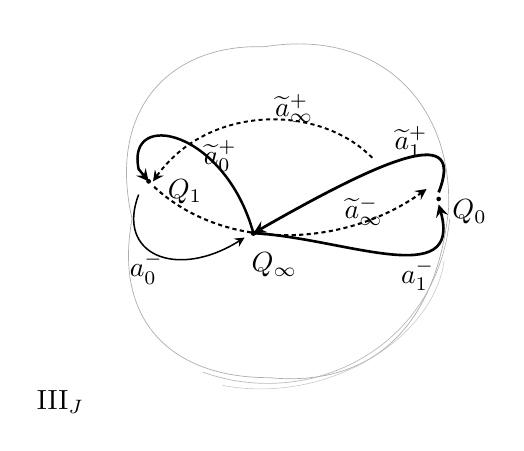
\begin{tikzpicture}[x=.014cm,y=-.014cm,>=stealth]
\draw[gray!65,line width=.25pt] (48,173) .. controls (25,73) and (83,14) .. (168,17)
 .. controls (272,0) and (338,68) .. (335,163)
 .. controls (326,259) and (275,327) .. (172,317)
 .. controls (82,317) and (31,264) .. (48,173);
\draw[gray!55,line width=.25pt] (112,312) .. controls (210,347) and (324,290) .. (336,173);
\draw[gray!45,line width=.2pt] (130,324) .. controls (225,342) and (321,282) .. (331,211);
\coordinate (A) at (63,139);
\coordinate (B) at (158,186);
\coordinate (C) at (326,155);
\fill (A) circle (2.2);\fill (B) circle (2.5);\fill (C) circle (2.1);
\draw[->,line width=.9pt] (B) .. controls (132,92) and (42,73) .. (54,128) -- (A);
\draw[->,line width=.55pt] (54,151) .. controls (33,205) and (88,229) .. (150,190);
\draw[->,line width=1pt] (326,149) .. controls (350,88) and (282,115) .. (B);
\draw[->,line width=.95pt] (B) .. controls (238,190) and (348,239) .. (326,160);
\draw[<-,line width=.7pt,dash pattern=on 1.5pt off 1.2pt] (67,139)
 .. controls (117,69) and (219,68) .. (267,119);
\draw[->,line width=.75pt,dash pattern=on 1.5pt off 1.2pt] (68,144)
 .. controls (133,204) and (241,199) .. (315,146);
\node at (96,148) {$Q_1$};
\node at (177,215) {$Q_\infty$};
\node at (354,167) {$Q_0$};
\node at (128,116) {$\widetilde a_0^+$};
\node at (61,218) {$a_0^-$};
\node at (301,103) {$\widetilde a_1^+$};
\node at (307,224) {$a_1^-$};
\node at (195,73) {$\widetilde a_\infty^+$};
\node at (258,166) {$\widetilde a_\infty^-$};
\node at (-17,339) {$\mathrm{III}_J$};
\end{tikzpicture}}

Le groupe $\{1,\tau\}$ y opère dans le graphe avec relations, par
\[
(27)\qquad\tau Q_i=Q_i,\quad\tau\widetilde a_i^\omega=(\widetilde a_i^{\omega'})^{-1}
\]
La donnée d'un \deleted{\unsure{autom.}} \inserted{endom.} du groupoïde $\widehat{\mathrm{III}}_J$, fixant les sommets et commutant à $G_J$, équivaut à celle d'un $\widetilde\alpha\in\widehat\Pi_{0,3}$, \deleted{$\unsure{\gamma|\lambda}\in\widehat{\mathbb Z}$}, satisfaisant \deleted{\unsure{l'équation rel.}} $(26)$. On aura, en introduisant
\[
(28)\qquad\widetilde\lambda_i^\omega=\widetilde a_i^{\omega'}\widetilde a_i^\omega,\in\deleted{\unsure{Q_{\omega'i}}}\inserted{\pi(Q_{\omega'i})}
\]
(\unsure{comparer à la définition dans le groupoïde} $\mathrm{II}_J$ ! $\lambda_i^\omega=\overset{\unsure{\deleted{\sim}|\sim}}{a}_i^{\omega'}a_i^\omega$)

\figure{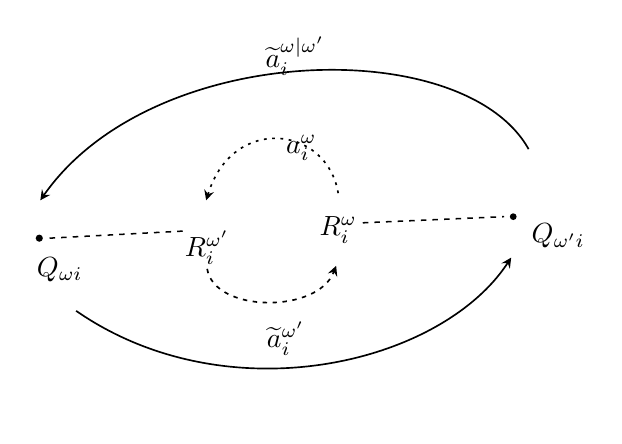
\begin{tikzpicture}[x=.013cm,y=-.013cm,>=stealth]
\fill (22,194) circle (3.5);
\fill (485,173) circle (3.3);
\draw[->,line width=.6pt] (500,107) .. controls (437,-6) and (132,1) .. (23,157);
\draw[->,line width=.6pt] (58,265) .. controls (205,367) and (414,318) .. (483,213);
\draw[line width=.55pt,dash pattern=on 2pt off 2.2pt] (32,194) -- (164,187);
\draw[line width=.55pt,dash pattern=on 2pt off 2.2pt] (338,179) -- (476,173);
\draw[->,line width=.6pt,dash pattern=on 1pt off 2pt] (314,150)
 .. controls (303,84) and (211,73) .. (185,157);
\draw[->,line width=.6pt,dash pattern=on 1.6pt off 2pt] (186,224)
 .. controls (193,267) and (294,268) .. (312,221);
\node at (42,225) {$Q_{\omega i}$};
\node at (529,192) {$Q_{\omega'i}$};
\node at (186,203) {$R_i^{\omega'}$};
\node at (314,186) {$R_i^\omega$};
\node at (272,16) {$\widetilde a_i^{\unsure{\omega|\omega'}}$};
\node at (263,292) {$\widetilde a_i^{\omega'}$};
\node at (278,106) {$a_i^\omega$};
\end{tikzpicture}}

\margin{\deleted{il semblerait raisonnable de changer les notations $\widetilde a_i^\omega$ devenant $\widetilde a_i^{\omega'}$}\quad $*$ \unsure{obtenir}, \unsure{une définition des} $\psi_i^\alpha$ \unsure{qui} \unsure{donne} dans $(29)$ \unsure{ainsi}. \unsure{cf.} \unsure{voir} \unsure{plus bas}}
\[
(29)\qquad u(\widetilde\lambda_i^\omega)=\overset{*}{\psi_{\omega'i}^{\omega'}}(\widetilde\alpha\varepsilon_0(\widetilde\alpha))\widetilde\lambda_i^\omega
=\psi_{\omega'i}^{\omega'}(\widetilde\alpha\varepsilon_0(\widetilde\alpha)l_0)
\]
Dans le cas où $\widetilde\alpha$ provient de $\eta,\gamma$ par $(27)$, on aura
\[
(30)\qquad\widetilde\alpha\varepsilon_0(\widetilde\alpha)l_0=\eta^{-1}l_0^p\eta\qquad(p=2\gamma+1)\ ;
\]
\margin{27}
